\newcommand{\mysize}{\footnotesize}
\resizebox{\textwidth}{!}{
        \begin{tabular}{M{2.75cm}M{5.25cm}M{5.25cm}M{5.25cm}}%
        \hhline{====}
             Réponse   & Régime apérodique        ($\xi>1$)  & Régime critique ($\xi=1$) & 
                         Régime pseudo-périodique ($0<\xi<1$) \\[0em]
        \hline
        Réponse impulsionnelle & 
            \resizebox{0.9\linewidth}{!}{\begin{tikzpicture}
    \begin{axis}
    [   legend style={draw=none},
        axis line style = thick,
        xmin=0,
        xmax=12,
        ymin=0,
        ymax=0.3,
        xlabel={$t$},
        ylabel={$s(t)$},
        label style={font=\Large},
        grid=both,
        grid style={line width=.4pt, draw=black},
        major grid style={line width=.4pt,draw=black},
    ]
    \addplot[signalb,domain=0:12] {(1/(3.73-0.26))*exp(-x/3.73)-exp(-x/0.26)};
    \end{axis}
\end{tikzpicture}
} 
            {\mysize $$ s(t)=\dfrac{1}{\tau_1-\tau_2}\left(e^{-\frac{t}{\tau_1}}-e^{-\frac{t}{\tau_2}}\right)$$} &  
            \resizebox{0.9\linewidth}{!}{    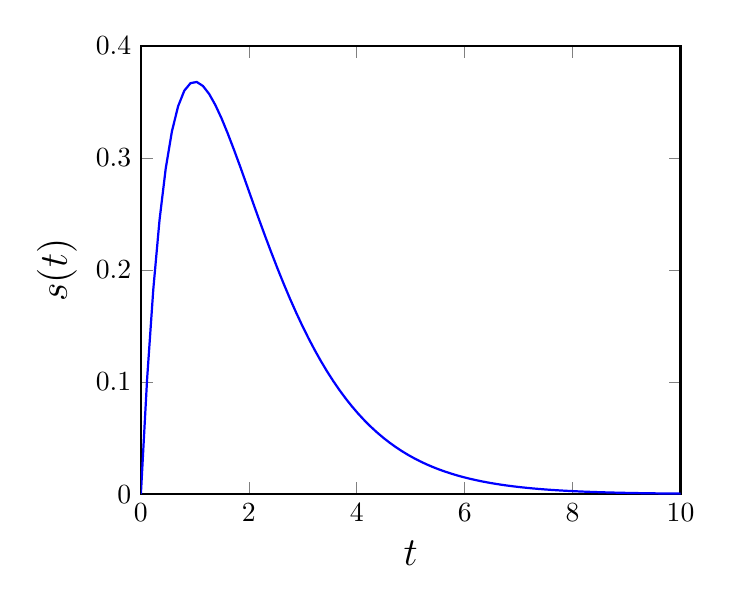
\begin{tikzpicture}
        \begin{axis}[
        legend style={draw=none},
        axis line style = thick,
        xmin=0,
        xmax=10,
        ymin=0,
        ymax=0.4,
        xlabel={$t$},
        ylabel={$s(t)$},
        label style={font=\Large},
        ]
            \addplot [thick,color=blue,domain=0:11.5, samples=101,unbounded coords=jump]{x*exp(-x)};
        \end{axis}
    \end{tikzpicture}
} 
            {\mysize $$s(t)=\dfrac{t}{\tau^2}e^{-\frac{t}{\tau}}$$} &  
            \resizebox{0.9\linewidth}{!}{\tikzsetnextfilename{2nd_rep_1_3_ext}
\begin{tikzpicture}
    \begin{axis}
    [   legend style={draw=none},
        axis line style = thick,
        xmin=0,
        xmax=12,
        ymin=-0.6,
        ymax=1.2,
        xlabel={$t$},
        ylabel={$s(t)$},
        label style={font=\Large},
        grid=both,
        grid style={line width=.4pt, draw=black},
        major grid style={line width=.4pt,draw=black},
    ]
    \def\a{0.3}            
    \def\b{0.91}           
    \def\w{0.953939201417} 
    \addplot[signalb,domain=0:12] {(\w/\b)*exp(-\a*x)*sin(deg(x)*\w)};
    \end{axis}
\end{tikzpicture}
} 
            {\mysize $$s(t)=\dfrac{\omega_d}{1-\xi^2}e^{-\xi\omega_0 t}\sin{\omega_d t}$$}\\[0em]
        \hline
        Réponse indicielle &  
            \resizebox{0.9\linewidth}{!}{\tikzsetnextfilename{2nd_rep_2_1_ext}
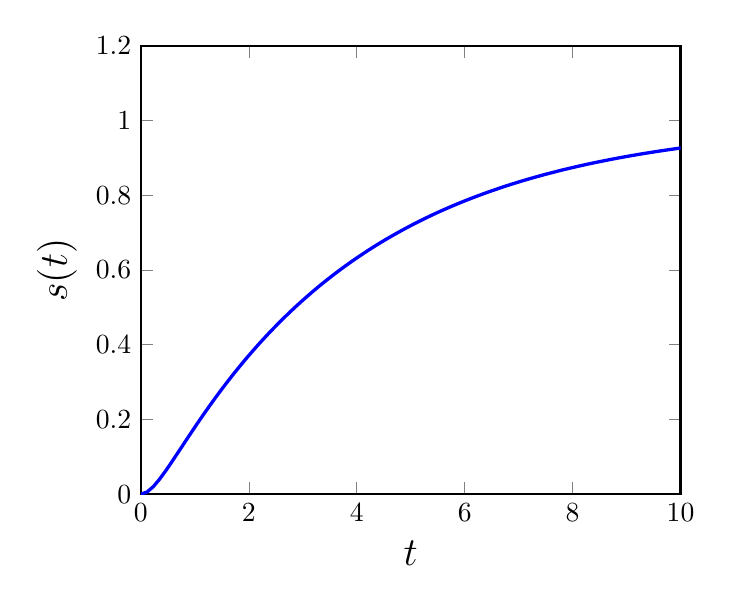
\begin{tikzpicture}
    \def\tu{2.0}
    \def\td{1.0}
    \begin{axis}
    [   legend style={draw=none},
        axis line style = thick,
        xmin=0,
        xmax=10,
        ymin=0,
        ymax=1.2,
        xlabel={$t$},
        ylabel={$s(t)$},
        label style={font=\Large},
    ]
    \addplot[very thick,color=blue,domain=0:11.5, samples=101]
    {1+(1/(3.73-0.26))*(0.26*exp(-x/0.26)-3.73*exp(-x/3.73))};
    \end{axis}
\end{tikzpicture}
} 
            {\mysize $$s(t)=1+\dfrac{1}{\tau_1-\tau_2}\left(\tau_2e^{-\frac{t}{\tau_2}}-\tau_1e^{-\frac{t}{\tau_1}}\right)$$} &  
            \resizebox{0.9\linewidth}{!}{\begin{tikzpicture}
    \begin{axis}
    [   legend style={draw=none},
        axis line style = thick,
        xmin=0,
        xmax=10,
        ymin=0,
        ymax=1.2,
        xlabel={$t$},
        ylabel={$s(t)$},
        label style={font=\Large},
        grid=both,
        grid style={line width=.4pt, draw=black},
        major grid style={line width=.4pt,draw=black},
    ]
    \addplot[signalb,domain=0:10]  {1-exp(-x)-x*exp(-x)};
    \end{axis}
\end{tikzpicture}
} 
            {\mysize $$s(t)=1-e^{-\frac{t}{\tau}}-\dfrac{t}{\tau}e^{-\frac{t}{\tau}}$$ } &  
            \resizebox{0.9\linewidth}{!}{\tikzsetnextfilename{2nd_rep_2_3_ext}
\begin{tikzpicture}
\begin{axis}
[   
    legend style={draw=none},
    axis line style = thick,
    xmin=0,
    xmax=12,
    ymin=0,
    ymax=1.5,
    xlabel={$t$},
    ylabel={$s(t)$},
    label style={font=\Large},
    grid=both,
    grid style={line width=.4pt, draw=black},
    major grid style={line width=.4pt,draw=black},
]
\def\a{0.3}            
\def\b{0.91}           
\def\w{0.954} 
\def\p{1.266}  
\addplot[signalb,domain=0:12] {1-((1./\w)*exp(-\a*x)*sin(deg(x)*\w+deg(\p)))};
\end{axis}
\end{tikzpicture}
} 
            {\mysize $$s(t) = 1 - \dfrac{e^{-\xi\omega_0 t}}{\sqrt{1-\xi^2}}\sin{(\omega_d t+\phi)}$$}\\[0em]
        \hhline{====}
        \end{tabular}
}

